\chapter{Phases}
During the development of the project, we decided to work in sprints, each lasting approximately two weeks, as discussed in \hyperref[devmethod]{\ref{devmethod} Development method}. However, it is apparent, in retrospective that our process can be divided into four phases:

\begin{center}
	\begin{tabular}{lcll}
		Phase 1 & - & Planning and research phase & week (1-4) \\
		Phase 2& - & Rest API and why it did not work with our project& week (5-8) \\
		Phase 3 & - & Websocket with SignalR & week (9-12) \\
		Phase 4 & - & Demonstration of our system & week (13-18) 
	\end{tabular}
\end{center}

An overview of our sprints are in figure \figref{fig:sprintoverview}
\section{Phase 1 - Planning and research phase}\label{sec:phase1}

After we had gotten in touch with Accenture and spoken with the supervisors and the product owner, the group had to make a few decisions regarding the project's direction.

An important choice for the project was to either build and train an AI model for the vehicles from scratch or use the existing model. Building a new AI model would provide a deeper understanding of the model we could utilize. However, we believed that our project would have the potential to be too similar to the previous project. Also, due to the time constraint, continuing with the existing model was more favorable. Our group also had more prior experience with networking than with Raspberry Pi and AI. We, therefore, chose to use the AI model from the previous project. 

In this phase, we did not have access to the vehicle, nor the code, made by the prior bachelor group. However, there was a need for project planning and research before we could start developing our IoT system. The topics that needed to be researched were:

\begin{itemize}
\item What causes traffic jams and solutions to fix it.
\item IoT-systems and how they function with vehicles.
\item Planning and development methods that will fit our project
\end{itemize}

We also used the pre-project phase to get to know Accenture, their guidelines, and their workspace.

%\subsection{Design thinking workshop}



\subsection{Choice of programming languages}
We chose to implement the client in Python and the server in C\#. The group before us had used Python for their Raspberry Pi vehicle, making Python a natural choice to extend the code from their project. Our group also had experience with networking in Python. Furthermore, the .NET ecosystem has well-developed solutions for creating IoT applications, microservices, and web applications \parencite{dotnet}. We had to write our server in C\#, to take advantage of these solutions. The server needed to be as efficient as possible, and C\# is also considered a fast programming language \parencite{csharp}. We also had some prior knowledge of coding in C\#.

\subsection{Internet of Things}

The Internet Of Things refers to physical objects that communicate using sensors, cameras, software, or other technologies connecting and exchanging data. This communication takes place over the internet or other communication forms. The number of connected IoT devices in the world is increasing, and it is becoming a big part of society \parencite{iot_analytics}. IoT has also been evolving in recent years due to other technologies becoming more accessible, such as machine learning and the 5G network.

IoT projects can, for instance, be applied in climate surveillance systems, energy, or transportation. In this thesis we will explore the possibilities of using IoT in transportation, more specifically in personal automobiles. The convergence of these fields is more commonly known as IoV, Internet of Vehicles. An IoV system is a distributed system for wireless communication and information exchange between vehicles through agreed-upon communication protocols \parencite{chinese_iov}. The system could potentially integrate functionality for dynamic information exchange, vehicle control and smart traffic management. In our thesis, we will explore these possibilities on a small scale.

\subsection{System security}
Security and privacy are important topics for any IoT system. Because these systems gather and work with vast amounts of data, they are naturally prone to be attacked. Moreover, as the systems grow and become more interconnected, with many devices worldwide, the imposed risk of such an attack increases drastically \parencite{iot_risk}. Anonymization of personal data, securing connections, and an intruder detection system are all security measures that require attention. The cars must be able to drive both with or without the system, which is an essential feature of system security. If there is a need for the server to shut down, the cars would need to be able to drive independently of the system. However, this project does not focus on these security measures due to time contraint. 

\subsection{Preventing traffic congestions for a one-lane road}\label{sec:traffic_congestion}

Traffic congestion, also known as traffic jams, is when a long line of vehicles moves slowly or has stopped moving altogether. Traffic jams can create frustration and disrupt nearby local environments with sound and gas emissions \parencite{traffic_congestion_pollution}. Many factors can cause traffic congestion, such as:

poorly designed roads, not wide enough roads, traffic light patterns, and accidents \parencite{traffic_congestion}.

With this in mind, we started by focusing on a simple scenario: when a car drastically reduces its speed or completely stops on a single-lane road.

This scenario will lead to the vehicles behind needing to slow down drastically as well. This phenomenon is called traffic jam shockwave \parencite{traffic_shockwave}. To prevent this, we propose a solution where cars reduce their velocity before they reach the destination of where the shockwave started. For this to happen, a server could keep track of the cars' positions and send information to the vehicles behind, when required. 

We came up with an idea on how the server and cars should interact. First, the car would connect to the server and provide information about its current speed, weight, width, and length. The server would use this information to keep track of all the cars' positions on the road. The cars would send information to the server if their velocity changed. This message would trigger an event on the server where it would command all the cars behind to slow down accordingly. \figref{fig:diagramfirst} shows a flow chart of a potential simulation of this solution:

\begin{figure}[h!]
	\centering
	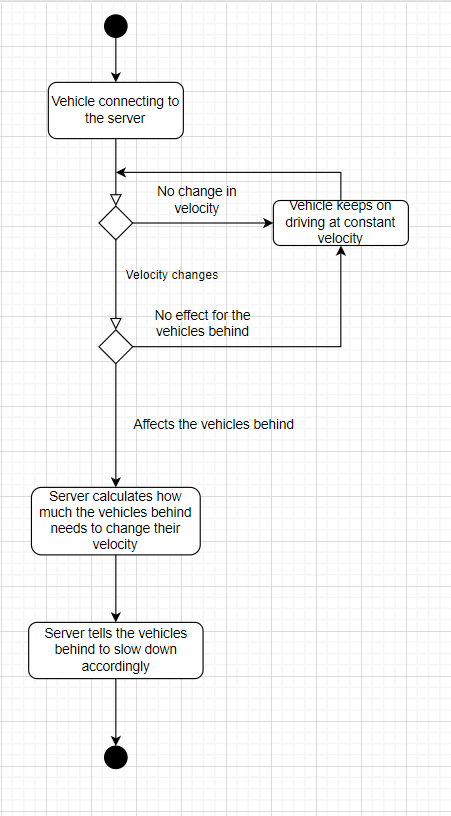
\includegraphics[width=0.9\linewidth]{figures/flow_diagram_first}
	\caption[Flow diagram server]{This figure shows the flow diagram of our first proposed solution. }
	\label{fig:diagramfirst}
\end{figure}
\clearpage
%\section{Implementation of Server and Client}
As IoT-systems become more complex, there is a need to structure them in layers. The three fundamental layers to an IoT-system consists of the perception layer, network layer and application layer \parencite[pp. 347-352]{iot_gateway}. In this part we will discuss what our things-layer and network-layer consists of, and explain the theory behind our decisions. 

\subsection{Implementation of Client}
Raspberry Pi is a small single-board desktop computer that is commonly used for IoT-projects. There is an enormous ecosystem of compatible devices that allow these computers to interact with the world in various ways. The organization states that they can be used for everything “from music machines and parent detectors to weather stations and tweeting bird houses with infra-red cameras” \parencite{raspberrypi}.  For our project we have used a Raspberry Pi Model 4, which the previous group used in their project. This is the newest and fastest model, which makes our test results as accurate as possible.  

The perception layer is responsible for perceiving the world, and creating data for the network layer to collect and deliver \parencite[pp. 8-9]{iot_platforms}. Devices that contribute to this are, for example, Global Positioning Systems(GPS), cameras and sensors. The raspberry-pi models we worked with utilizes both a camera and a range detection sensor that gets processed by the image recognition algorithm running on the machine. These vehicles play the role of client in our system, as they connect to the server. 

The requirements for our client was that it needed to be able to take in commands from the server and respond correctly to those commands. In addition, they had to be able to act by themselves if they were not connected to the server. For that to happen the vehicles had to send their size, position and velocity to the server when they connected initially. The server also needs to send their velocity and position to the server at a frequent rate so that the server can keep track of that information.
\subsection{Implementation of Server}
The network-layer of an IoT-system is responsible for transferring data collected by the things-layer \parencite[pp. 8-9]{iot_platforms}. In our project this is done by a centralized server that is connected to all the clients. 

The task required the client, which in our case is the cars, to receive the commands from the server. The group prior had made it such as the car made decisions based on its AI. The AI used picture recognition which could recognize speed limit signs and stop signs. The cars were also programmed to follow a path. Furthermore we needed a server which could send commands to the clients at a frequent rate, based on the information given by the clients. The server’s commands need to overwrite the AI that is already on the vehicles.

Here are some requirements needed for the server:
\begin{itemize}
	\item Needs to be able to send messages to all clients simultaneously, or a specific group of clients.
	\item Handle increasing traffic
	\item Little to no delay
	\item Two way communication between server and client
\end{itemize}

We initially coded a server by using API. The server was able to receive information from the clients, but for the cars to receive information from the server, they had to host their own servers. The car’s main priority should be calculating decisions based on their AI, not hosting a server. It would also be harder to add a server to the code from the previous group. We therefore thought of some other solutions. 

Websockets provides a two way communication over a single tcp-connection. This means that both the server and client can send and receive messages from each other. They also allow for a better efficiency than REST API because they do not require the request/response overhead for each message that is sent and received. This solved the issue we previously had with the solo API-solution.

ASP.NET Core Signal R is an open source library that simplifies adding real-time web functionality to apps (Microsoft, 2022). It supports websockets as a real time communication which is perfect for a two way communication. Signal R is often used in games, social networks and gps-apps where information to the clients are needed instantly. It also scales with increasing traffic. Signal R uses hubs where servers and clients communicate with each other. Hubs allows servers and clients to call methods on eachother. Since the server needs to send the cars commands this is perfect for our Iot-system.

The server needed some specific functionalities in correlation with the problem statement stated earlier. We did some research on what caused traffic jams and chose two problems which our server would focus on solving:

\begin{itemize}
	\item Delayed reaction times when people stop and accelerate 
	\item Increased traffic flow in intersections
\end{itemize}

The first point happens when a car changes velocity. Therefore the server has to check if any car’s have changed their velocity. If yes, the server needs to send a command to all the car’s behind a certain distance of the car that changed their velocity.  The distance will be calculated by the server based on the change of velocity. The command sent out to the car’s behind will be to change velocity based on distance to the car that changed their velocity and the amount of changed velocity.

To increase traffic flow in intersections we can have the server work as some traffic lights. The server can check if cars are closing in on the intersection’s position and give one lane the green light and the other the red light. The lights will depend on which car’s come first. The difference between a server doing this and a traffic light system is that the server can tell the vehicles to slow down before the intersection, making the traffic flow smoother.
%\section{Implementation of simulation}
To show that the solution was reaching the requirements we needed to create a demonstration. A demonstration was also an important part of testing the functionalities of the IoT-system. There were two options which were viable in this case. The first one was to create a virtual simulation using unity or another graphic-program. The other option was to build a physical demonstration with two or more cars. We chose to implement a physical demonstration with two cars. This was because we already had one car finished by the previous group. In addition it was more beneficial for Accenture with a physical demo since they can show it at exhibits.
\begin{itemize}
	\item That the server can turn off and the cars would still drive on their own.
	\item Cars communicating through the server and acing based on the server’s decisions
	\item Scalability to the real world
\end{itemize}
First we built the server with only one single lane road in mind. With this solution the potential of showing off the functionalities of the IoT-system was low. We could potentially have shown that if a car in front slows down, the car behind also slows down. This would show that the system could prevent some traffic, but only in a specific scenario. However we wanted to show that the IoT system could work in more than just one single-lane road. We therefore chose to try to emulate an intersection in the physical demo.

For a physical demo to work we needed to build another car. Luckily the previous group had documented their work and we could follow their process from their final report. We also had the parts provided to us. However we were unable to get the full functionality of the second car since the TPU accelerator used by the previous group was unavailable. The TPU accelerator provided the car with the processing power needed for the AI. This meant that the car was built without the camera. But this had a minor effect on our demo since the other car was fully functional without the system. We solved this problem by letting the server do the decision making for the car with less functionality.

We also needed to emulate a road system which contained the intersection we were going to demonstrate in the demo. Since the AI had not trained to recognize intersections yet we had to code a road system into our server that contained roads, lanes and intersections. We then had to build a physical intersection for our cars with tape that correlates with the emulated intersection. 

\subsection{Calibration of the cars}
When the server, vehicles and client were implemented, and the second vehicle built, we did some testing to figure out how the car’s behaved when given directions by the server. In this test the vehicles were given a specific velocity and driving distance by the server. When the vehicles arrived at their destination the server would tell them to stop. The car’s drove in a straight line.

The vehicles were able to send information, and respond correctly to the servers commands. We also observed that the vehicles drove a different length for each velocity given even though the length was the same. This is because the velocity given to the vehicles is the amount of power going into the car’s motors, not the actual velocity of the car’s. We wanted the demo to be accurate so our group did some further testing where we wrote down the results. 

\begin{table}
	\begin{center}
		\begin{tabular}{rrrr}
			\hline
			Power (?) & Length (cm) & Time (s) & Velocity (cm/s) \\
			\hline
			40 & 467 & 8.98 & 52.00 \\
			50 & 425 & 7.28 & 58.38 \\
			60 & 400 & 6.06 & 66.01 \\
			70 & 357 & 5.18 & 68.92 \\
			80 & 325 & 4.49 & 72.32 \\
			90 & 314 & 4.03 & 77.92 \\
			100 & 286 & 3.62 & 79.01 \\
			\hline
		\end{tabular}
		\caption{Test text}
	\end{center}
\end{table}

The data Power was the velocity given by the server. Velocity was the actual velocity in our testing, which is length divided by time. As you can see the velocity was not the same as the power. We then made a graph to visualize the two values. The $y$-axis was the velocity while the $x$-axis is the power.

\begin{figure}[h!]
	\caption{Graph of velocity as a function of power}
\end{figure}

We observed that the correlation between power and velocity seemed linear. This means we could make a specific formula that describes the correlation between the two values. We used linear regression to figure out this formula:

\begin{figure}[h!]
	\caption{Graph of velocity as a function of power with linear regression}
\end{figure}

The formula we ended up with was as follows: $P = 0.4516v + 36.189$, where $P$ is power and $v$ is velocity, with a mean square error of $R^2=0.9653$. When we coded the formula into the vehicles we did another set of testing. We observed that the vehicles drove more or less the same distance for each power given. If we wanted an even more accurate formula we could have tuned the formula with the test results from our new test. Although the results were not hundred percent accurate, we concluded it was accurate enough for our demonstration. 

To test the solution we have worked on, we made a physical demonstration with two cars that meet at an intersection, as part of the product documentation. We want to test that a combination of a centralized communication system and artificial intelligence can improve traffic flow. What we wanted to observe was if the velocity of the vehicles were not drasticly changed and therefore not distrupting the traffic flow.


%\subsection{System security}
Security and privacy are important topics for any IoT system. Because these systems gather and work with vast amounts of data, they are naturally prone to be attacked. Moreover, as the systems grow and become more interconnected, with many devices worldwide, the imposed risk of such an attack increases drastically \parencite{iot_risk}. Anonymization of personal data, securing connections, and an intruder detection system are all security measures that require attention. The cars must be able to drive both with or without the system, which is an essential feature of system security. If there is a need for the server to shut down, the cars would need to be able to drive independently of the system. However, this project does not focus on these security measures due to time contraint. 

\section{Phase 2: REST API}\label{phase2}
The aim of the project was to connect Raspberry Pi devices to a system. Thus, the group decided that the best way to establish this connection was to implement a RESTful API on the server. In addition, the question on how the data should be stored was also arises during this phase.

\emph{Representational state transfer} (REST) \emph{application programming interface} (API) provides a way for client and server to establish communication through \emph{hypertext transfer protocol} (HTTP). Using a REST API clients can send requests to a server to perform standard CRUD (create, read, update and delete) operations on a database \parencite{rest_api}.

Due to the time sensitivity of the application we are trying to build, it was therefore necessary to choose an appropriate type of database for our system. In this case, we chose to incorporate the time series database. InfluxDB is a time series database created by InfluxData. It provides a SQL-like syntax for querying resources that is quick and scalable, and most importantly free. Moreover, InfluxDB client library, using the influxDB v2 API, provides both ease of install and use for a multitude of langauages \parencite{influxdb}.

During this phase the group implemented a standard REST API server with C\# with the idea that the Raspberry Pi vehicles should exchange information on its velocity, acceleration and position to the server. Client should first POST itself to the server. The server will then add the vehicle to the influxDB to keep track of the vehicle's information. Then, the vehicle should be able to perform a GET request to the server to retrieve its information.

The client at this phase would be able to send a PATCH request to the server in order to update its information. In addition, the server will add a new entry into the database whenever it receives this request. The idea was that the client and server would be able to continuously communicate to each other such that the server could determine the behaviour of all connected clients.

However, a RESTful API server were not able to perform all its required task that the group wanted the server to do. Firstly, the server were only able to communicate with one client at the time, i.e. the client that sends a request. What the group wanted at this stage was that based on a request the server should also be able to send its own request to all the other clients. In order to acheive this, the server had to send an unprompted response to other clients that is not requesting a resource from the server, which was not possible with our current architecture.

A new solution had to be in place in order to achieve our goal. Other solutions were proposed during this stage.

\subsubsection*{Long polling}
Polling is the idea that the server pushes resources to the client. There are mainly two types of polling; short- and long polling. 

In short polling, a client requests a resource from the server and the server responds with nothing if the resrouce is not available. The client will then send a new request in a short amount of time and the cycles repeats until the client receives the resource it has requested.

Long polling is similar to short polling, however, the server does not send anything back before the resource is available. That is, the client sends a request to the server and the server is holding this request until it has a response available to the client. In our case, we wanted every client to perform a GET request to the server on a seperate thread and instruct the server to hold onto this request until it had further instructions to the requesting client.

However, implementing a method on the server to block the response introduced more complication to the project. Also, with the asynchronous nature of the controllers implemented on the server it would also mean that the server will consume a lot of the processor which also means that the performance of the server will be heavily deteriorated.

\subsubsection*{Implement REST API on the client}
Another solution was to implement the client itself as a REST API server on its own. However, in order to achieve this, each client needed to also send the server its host and port information to the server. Also, the server has to be implemented as a client in order to connect to the vehicles.

\subsubsection{Webhooks}
Webhooks, according to \cite{webhooks}, is a user-defined callback over HTTP. In our case, implementing webhooks to post notifications on clients based on events sent to the server. This was a good contender to solve our issue. However, implementing webhooks includes extensive research into a system the group had never heard of, in addition to scarce information on how to create such a system. The group decided that the time constraint of this project did not justify the time it would take to implement such a system.

\section{Phase 3 - Websocket with SignalR}\label{phase3}
After extensive research on how to solve the two-way communication discussed in \secref{phase2}, the group agreed that WebSockets would be an excellent solution to our problem. Using WebSockets, both client and server can transfer data whenever they see fit. However, \cite{microsoft_websockets} discourages developers from implementing raw WebSockets for most applications and recommends using SignalR instead.

ASP.NET SignalR is a library that at the top layer provides real-time communication using WebSockets while also providing other transport methods such as long-polling as fallback \parencite{microsoft_signalr}. Furthermore, SignalR API supports \emph{remote procedure calls} (RPC) using hubs, meaning we can invoke subroutines on the client from the server and vice versa \parencite{microsoft_signalr}.

As a result of the failure to attain the result we wanted with REST API and InfluxDB, as discussed in \secref{phase2}, we decided to implement SignalR without InfluxDB on our server instead. First, set up an echo server using SignalR while simultaneously implementing the client code. The client code had to be implemented independently of the Raspberry Pi code. Because our goal was to create a communication module that is reusable through inheritance for other devices, e.g., traffic lights, should it be required to set up a new hub with other devices.

After successfully implementing all the necessary methods on the client, the vehicle class representing the Raspberry Pi device became our next priority. By inheriting the client class, the vehicle class also inherits its ability to connect, listen and send data to the server. Furthermore, the client can also subscribe to events that the server can trigger using RPC.

\subsection{Implementation of traffic on a single lane}
After witnessing a successful connection between the Raspberry Pi vehicle and our SignalR server, we started to implement the necessary functionality on the server. We started with the simple scenario described in \secref{sec:traffic_congestion}. The client will inform the server whenever its velocity has changed. Then, the server will relay this change to every other vehicle behind it on the same road and adjust their velocities accordingly. This server functionality also depends on the continuous monitoring of each vehicle's position. Thus, raising a new issue on how the vehicle information should be stored.

InfluxDB could, in theory, be used to store the vehicle's position; however, since the position is constantly changing, it would require the server to read and write on the database continuously. Hence, the group concluded that this would potentially impact latency on the server. Thus, we unanimously determined that a live-in-memory database storing vehicles in lists would be preferable. With simple mathematics, the server could recalculate the vehicle's position based on its previous velocity and a stopwatch whenever it retrieves the information about a vehicle instead.

We then determined to show the product owner from Accenture what we had been working on, thus inviting him and the external supervisor to the next meeting. This short demonstration consisted of running multiple clients with the server to simulate how multiple vehicles would behave with the intervention of our server. The simulation successfully demonstrated that vehicles were able to adjust their velocities in order to prevent the shockwave phenomena described in \secref{sec:traffic_congestion}, and we received positive feedback. However, our supervisors challenged us to extend our concept and make our solution more complex. They believed implementing an intersection where multiple cars meet could show more advanced traffic management. They believed implementing an intersection where multiple cars meet could show more advanced traffic management.

\subsection{Extending the concept to a more complex scenario - traffic on an intersection}
Expanding further on the concept, new functionalities on the SignalR server were developed to handle vehicles approaching an intersection. With a more complex topology, expanding the database to account for the new road network is also required. Consequently, roads and intersections became required additions to our solution. Furthermore, the vehicle model on the serverside is now also composed of a route planner to represent what it means to be approaching an intersection.

With these improvements and new functionalities, the server can command the clients to adjust their velocity to avoid collisions between vehicles approaching an intersection simultaneously. By reducing the velocity of some vehicles, it also became apparent that traffic flow is improved, in contrast to stopping a vehicle.
\section{Phase 4 - Making a demo}

At this point in the development we were sure about what kind of situation we wanted to simulate to make a satisfying product for Accenture, and to answer the problem statement we had decided on. Following the work requirements we now needed to make a demonstration that showed how the system worked. At this point we also decided that we wanted to make a physical demonstration instead of making a digital simulation, although this was a solution that would take less effort and still be a valid solution. At the start of this work phase we had started to consider making only a digital simulation, but after a meeting with our external supervisors at Accenture, in which we were advised that a physical demonstration was more in line with Accenture's goals for the project, we finally decided to make a physical demonstration. 

\subsection{Building a new car}
The previous group had only built one car for their project. Consequently, we needed to build a new car to show a situation where two cars meet at an intersection. Luckily, Accenture kept a box of unused components from the previous group. However, we only had one TPU, the Coral Usb Accelerator. The TPU is an essential component for giving extra processing power to the computer, and it was necessary to run the artificial intelligence the previous group had used \parencite{prev_project}. 

Without this accelerator, we could not run the artificial intelligence the previous group had incorporated into their solution due to the global chip shortage caused by the Covid pandemic; the accelerator was unavailable to purchase anywhere. As a result, the new car's camera and distance measuring sensor were absent. Not having two cars that utilized artificial intelligence could be a challenge. One of the required features of our solution was that the cars should be able to drive using the AI when a server connection was unavailable, as per described in \secref{sec:goals}. We decided that as long as we had one car that could navigate traffic independent of the server, the other car could drive solely on commands given by the server. With the components and the product documentation of the previous project \secref{sec:goals}, we were able to build a copy of the car as seen in \figref{fig:twocars}.

\begin{figure}[h!]
	\centering
	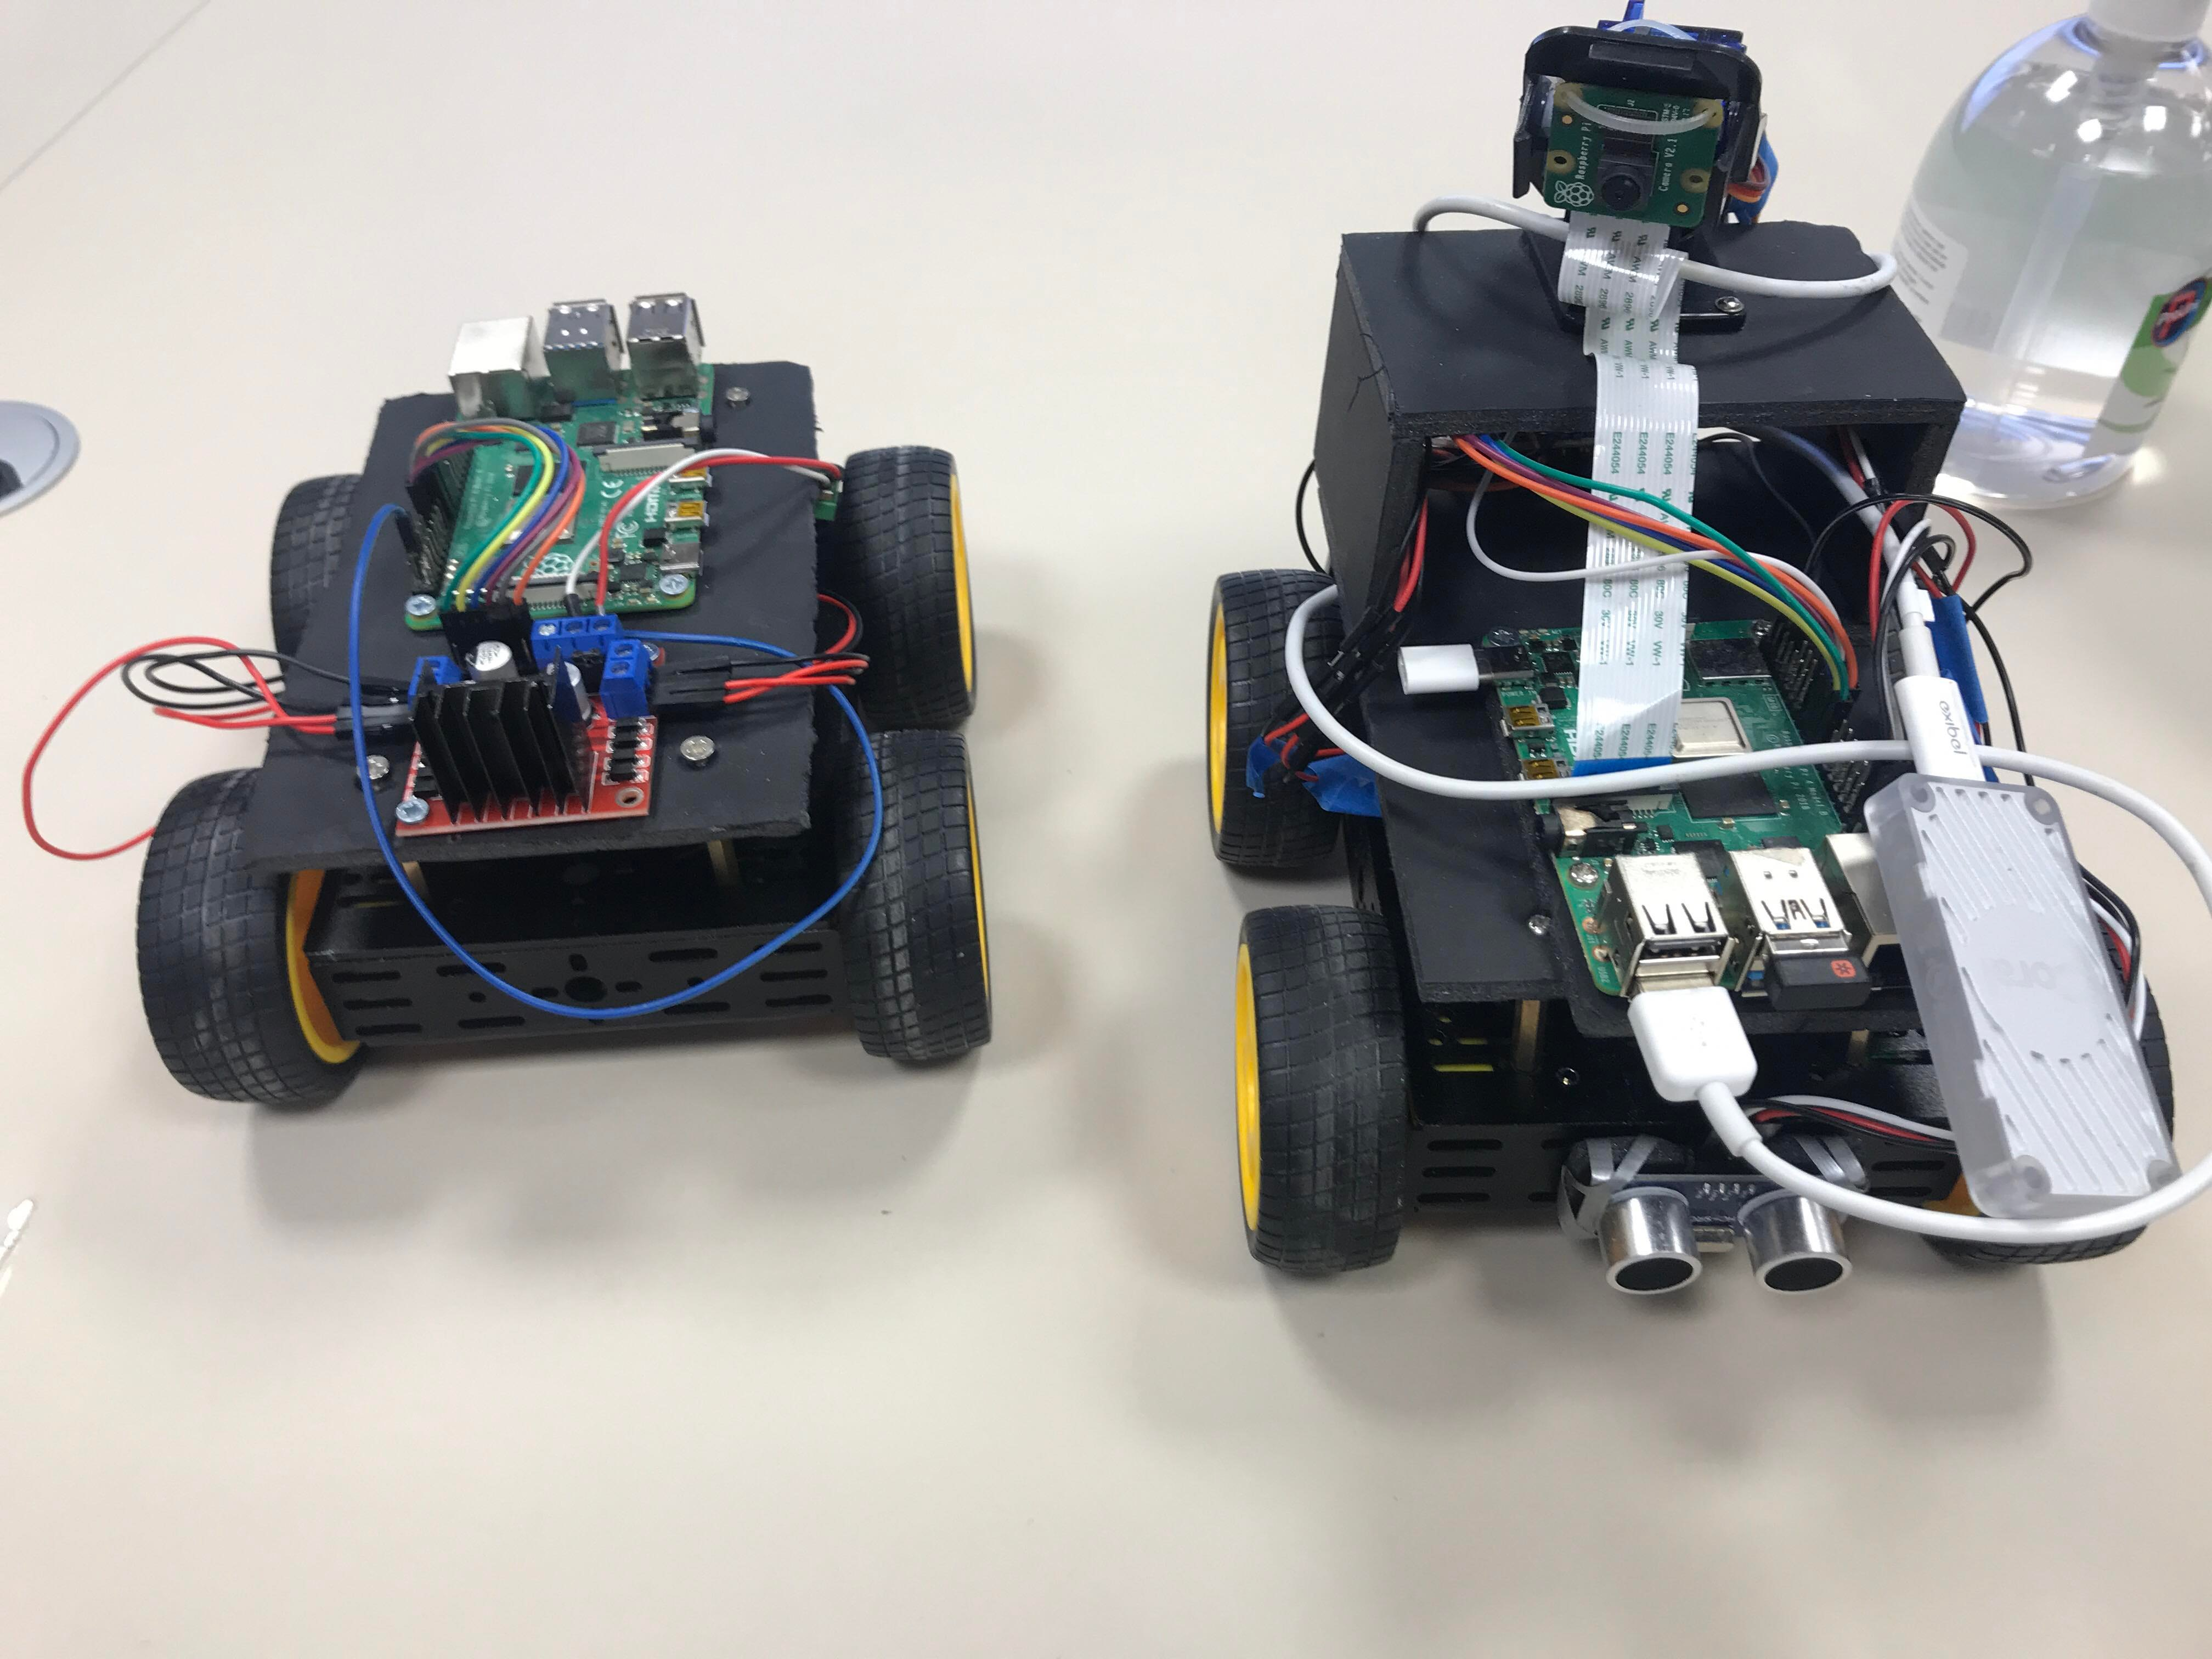
\includegraphics[width=0.9\linewidth]{figures/two_cars}
	\caption{Photo of the two cars we built. To the left is the car without a camera. To the right is the car with a camera on top and a Coral USB Accelerator Edge TPU. This car can take advantage of the onboard AI.}
	\label{fig:twocars}
\end{figure}




\subsection{Calibration of the cars}
When the server, vehicles and client were implemented, and the second vehicle built, we did some testing to figure out how the car’s behaved when given directions by the server. In this test the vehicles were given a specific velocity and driving distance by the server. When the vehicles arrived at their destination the server would tell them to stop. The car’s drove in a straight line.

The vehicles were able to send information, and respond correctly to the servers commands. We also observed that the vehicles drove a different length for each velocity given even though the length was the same. This is because the velocity given to the vehicles is the amount of power going into the car’s motors, not the actual velocity of the car’s. We wanted the demo to be accurate so our group did some further testing where we wrote down the results. 

\begin{table}
	\begin{center}
		\begin{tabular}{rrrr}
			\hline
			Power (?) & Length (cm) & Time (s) & Velocity (cm/s) \\
			\hline
			40 & 467 & 8.98 & 52.00 \\
			50 & 425 & 7.28 & 58.38 \\
			60 & 400 & 6.06 & 66.01 \\
			70 & 357 & 5.18 & 68.92 \\
			80 & 325 & 4.49 & 72.32 \\
			90 & 314 & 4.03 & 77.92 \\
			100 & 286 & 3.62 & 79.01 \\
			\hline
		\end{tabular}
		\caption{Test text}
	\end{center}
\end{table}

The data Power was the velocity given by the server. Velocity was the actual velocity in our testing, which is length divided by time. As you can see the velocity was not the same as the power. We then made a graph to visualize the two values. The $y$-axis was the velocity while the $x$-axis is the power.

\begin{figure}[h!]
	\caption{Graph of velocity as a function of power}
\end{figure}

We observed that the correlation between power and velocity seemed linear. This means we could make a specific formula that describes the correlation between the two values. We used linear regression to figure out this formula:

\begin{figure}[h!]
	\caption{Graph of velocity as a function of power with linear regression}
\end{figure}

The formula we ended up with was as follows: $P = 0.4516v + 36.189$, where $P$ is power and $v$ is velocity, with a mean square error of $R^2=0.9653$. When we coded the formula into the vehicles we did another set of testing. We observed that the vehicles drove more or less the same distance for each power given. If we wanted an even more accurate formula we could have tuned the formula with the test results from our new test. Although the results were not hundred percent accurate, we concluded it was accurate enough for our demonstration. 

To test the solution we have worked on, we made a physical demonstration with two cars that meet at an intersection, as part of the product documentation. We want to test that a combination of a centralized communication system and artificial intelligence can improve traffic flow. What we wanted to observe was if the velocity of the vehicles were not drasticly changed and therefore not distrupting the traffic flow.


\subsection{Construction of semi physical demonstration}\label{sec:demo}
We wanted to test that a centralized communication system and artificial intelligence could improve traffic flow. In order to test the solution, we made a semi physical simulation where two cars approach an intersection simultaneously. We wanted to observe if the velocity of the vehicles were not drastically changed and, therefore, decreased shockwave described in \secref{sec:traffic_congestion}.

We found a space at Accenture that was big enough to build the track. The power input on the Raspberry Pi vehicles is limited to between 40 and 100 units. Since the server will adjust the vehicle's speed to avoid a collision, the intersection was required to be at least 130cm away from the starting point to prevent the server from adjusting speed outside the equivalent power limit. Furthermore, the server prevents cars from driving before at least two vehicles have established a connection. Hence, both vehicles will start their journey simultaneously. We also placed the vehicles at the same distance from the intersection on their respective roads. Given these initial conditions, both vehicles are supposed to collide without the server's intervention. We also made the server log the velocity sent to the cars to track how much the cars' velocities changed.

Making the demo one hundred percent accurate was not possible in our circumstances due to the limitations of the Raspberry Pi. Furthermore, the vehicles were not able to receive the messages simultaneously. Consequently, this meant that they could start with a minor time difference. Another factor was that the trajectory of the vehicles was not always straight. However, we were able to get a consistent demo with enough margins. \figref{fig:crashdemo} shows an example of a collision during a test demonstration.

\begin{figure}[h!]
	\centering
	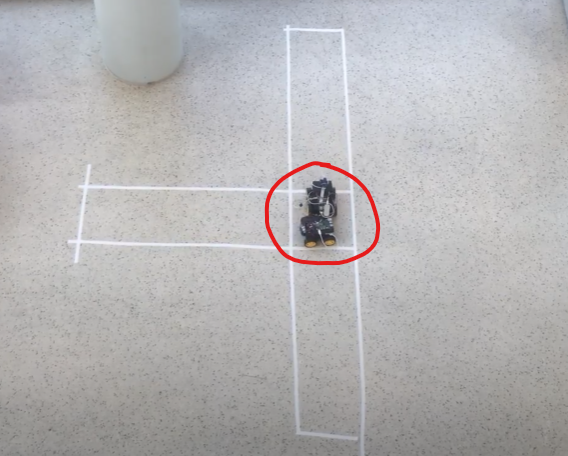
\includegraphics[width=1\linewidth]{figures/demo_crash}
	\caption{Here, we can observe the two cars colliding in the intersection. One of the cars started about 5 centimeters further behind the other car and started a few milliseconds later, resulting in a collision. Meanwhile, the server assumed they started simultaneously at the same distance from the intersection.}
	\label{fig:crashdemo}
\end{figure}

Furthermore, the server did not account for the lengths of the vehicles during its calculations. After we introduced the length of the vehicles and buffer zone, we were able to get a consistent semi-physical demonstration.

When both vehicles had connected to the server, the cars would drive with an initial speed of 80 cm/s, the upper limit of the Raspberry Pi. Not long after they started to drive, the server recognized the cars approaching the intersection. The server calculates using the car's velocity, position, and length. Then the server calculates which car has to slow down and how much the car needs to slow down to avoid a collision, in this case, to 55 cm/s. After the other car has supposedly passed the intersection, the car that slowed down gets told by the server to speed its velocity back to 80 cm/s. \figref{fig:successdemo} is a snapshot of a successful test demo.

\begin{figure}[h!]
	\centering
	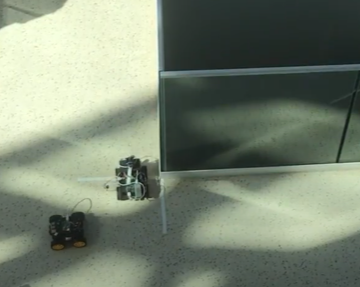
\includegraphics[width=1\linewidth]{figures/succsess_demo}
	\caption[Successful demo]{Here is a snipped from a successful demo. The car to the left has just passed the intersection, marked as a square with white tape. The car furthest up is, therefore, about to adjust back to its original velocity. Here we can observe that the server prevents a collision.}
	\label{fig:successdemo}
\end{figure}
%\input{chapters/sections/subsections/building_road_model}
%\input{chapters/sections/subsections/simulating_situation}


\section{Results}

We observed troughout multible demonstrations that the vehicles accelerated from 80 cm/s to 55 cm/s when the server intervined. Without the servers intervention, one of the vehicles would have had to completely stop at the intersection which would be a higher change in velocity. We concluded with that in this specific scenario, the server had increased traffic flow. However it is hard to say anyhting regarding more complex scenarios with more vehicles.

\section{Evaluation of process}
In our process documentation we have described the way the project progressed from beginning to end. In this section we will discuss positive and negative takeaways, with the goal of aiding further work on the project. This will include our approach to work methodology, communication and team building. 

\subsection{Work methodology}
As previously mentioned, we chose to apply an agile work methodology based on the fact that our project seemed to be prone to many changes. We included rituals like daily stand-ups, sprint planning meetings and retrospective meetings after sprints. Doing this helped our team understand what difficulties the other members were facing, and gave us time to discuss our obstacles daily. 

There were also some elements of agile development that we did not incorporate, either because of lack of experience or lack of time. As explained in the work of  Skyttermoen, T. and Vaagasar, A.L.; agile development teams regularly have meetings with the product owner, who give feedback on the strengths and weaknesses of the deliveries \textcolor{red}{(Skyttermoen \& Vaagaasar, 2017, pp.120)}. Our group only had a few meetings with the product owner during the project period, to update him on how far along we were. We did, however,  have biweekly meetings with our external supervisors at Accenture who provided us feedback on the work we had done. Because we had the freedom to choose the type of solution we wanted, as long as it met the requirements that were set to us, we didn’t need the product owner to be in our biweekly meetings. 
\subsection{Possible improvements}
All the features in the MoSCoW method from \secref{sec:moscow_method}, "could have" to "won't have this time" are features for a future project, either for Accenture to improve or for a future bachelor project. Although it fulfilled the product requirements given by Accenture, there is room for improvement. For example, with the accuracy of the demo, specifically by doing more calibration tests and making a more accurate formula than we were able to produce (see \hyperref[eq:vprelationship]{equation \eqref{eq:vprelationship}}). Furthermore, changing the wheels and installing an edge TPU to exploit the existing AI model will result in a more predictable trajectory of the vehicles.

Our demo only contains two cars, but our server supports scenarios with multiple cars. There are also possibilities to connect other devices to the server, for example, traffic lights. However, there are no specific functionalities for other IoT devices on the server. Scaling the IoT system for functionalities with other IoT devices is a task for future development. Adding roads and making a more complex road system would also be a task for future development.

As mentioned, we made a semi-physical simulation. However, a virtual simulation would potentially yield more data for research while also exploring other more complex road configurations.

Due to this project's time constraints, we, for instance, did not integrate machine learning with our server. Integrating machine learning on the server could expand its different capabilities and make the project more scalable and applicable to a broader range of scenarios. Such integration is deemed valuable for the further extension of this project.

Making a viable product in the real world is a long way ahead and will require a lot more testing and implementation on a bigger scale. With the rise in availability of self-driving vehicles and the 5G network, there could be a possibility of IoT systems managing traffic. We explored the posibility of implementing multiple servers, each  having responsibility for their own geographical area, or an entire road. This follows the edge computing architecture, which is popular in IoT systems and describes distributed network devices that communicate to one centralized server through ``edge'' devices \parencite[pp 149]{iot_platforms}. We did not implement this in our program, but it was one of our main ideas for how we would scale the system to implement more roads.

Finally, we hope that our testing and research can be of value towards realizing autonomous cars and traffic management on such a scale.

